\section{THIẾT KẾ MÔ HÌNH MẠNG}

\subsection{Sơ đồ tổng thể}

Topology tổng thể gồm ba chi nhánh doanh nghiệp kết nối vào provider backbone. Mỗi chi nhánh có CE riêng; mỗi CE kết nối đến một PE tương ứng; các PE kết nối qua nhóm P router trong lõi provider.

\begin{figure}[H]
    \centering
    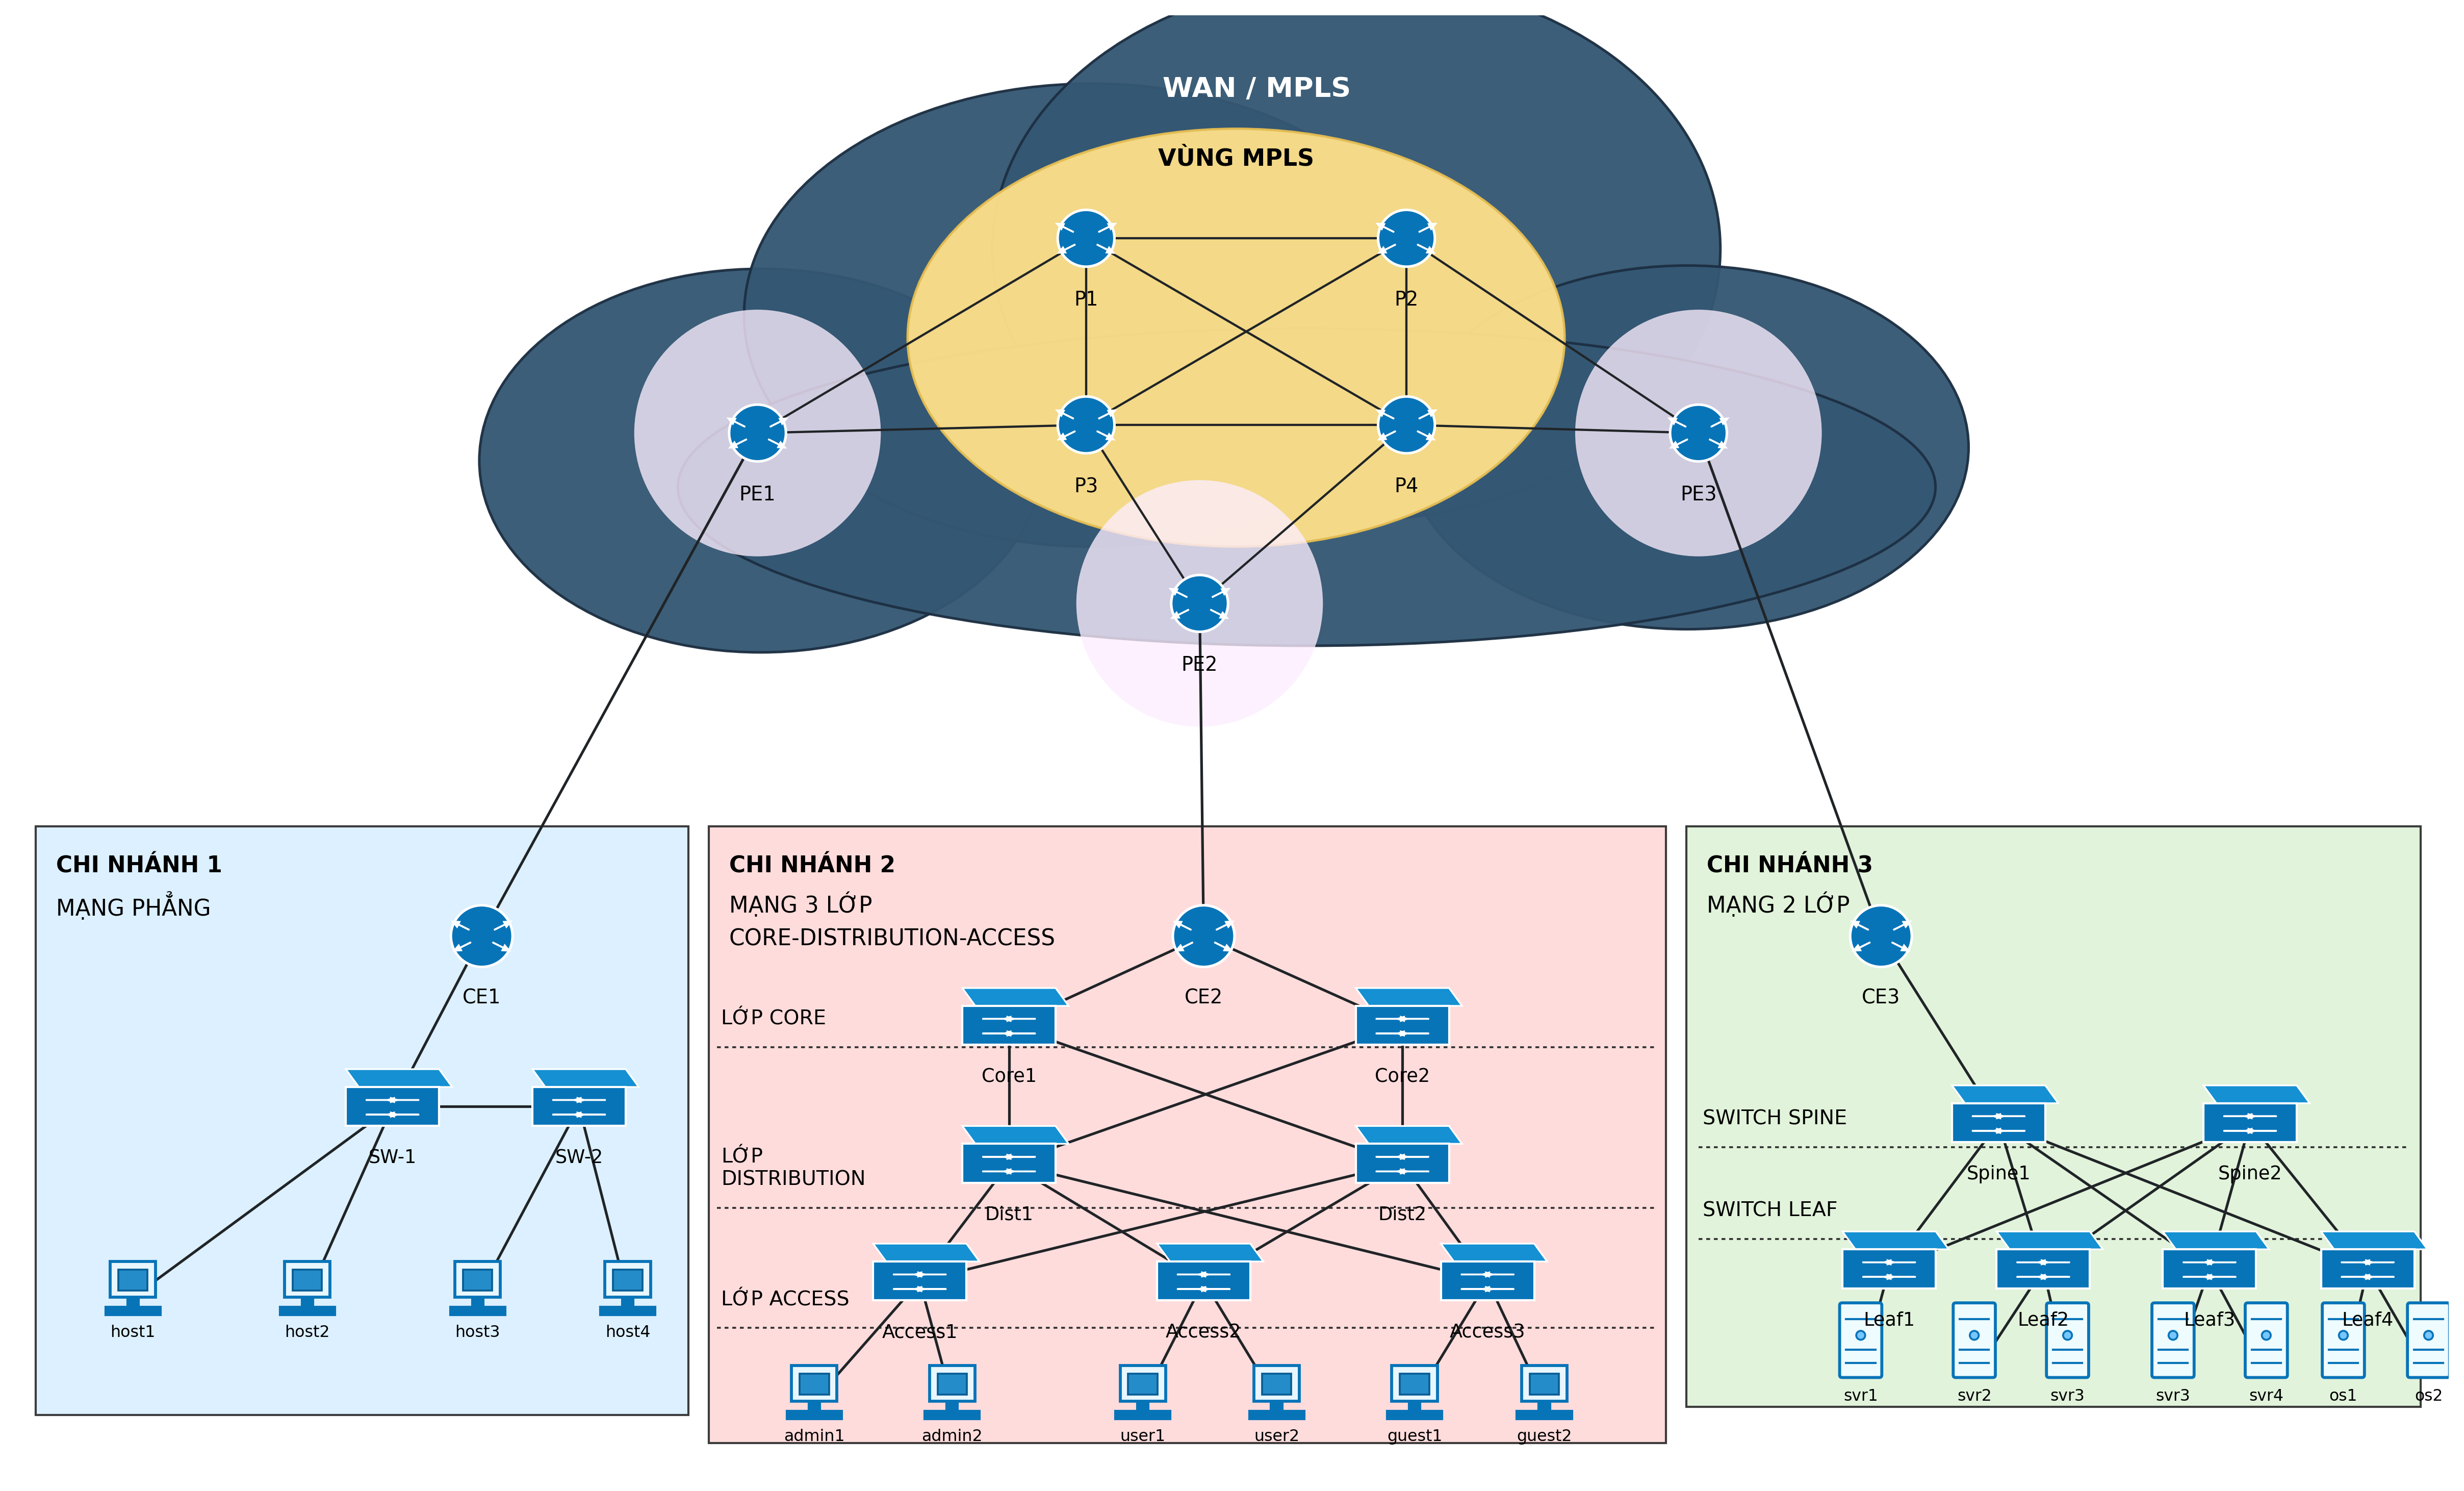
\includegraphics[width=0.95\linewidth]{image/topology_overview.png}
    \caption{Sơ đồ tổng thể Metro Ethernet MPLS}
\end{figure}

\subsection{Thiết kế Branch 1: Flat Network}

Branch 1 có bốn host \texttt{host1}, \texttt{host2}, \texttt{host3}, \texttt{host4}, hai switch access và CE router \texttt{b1\_ce}. Các host dùng subnet \texttt{10.1.0.0/24}, gateway là \texttt{10.1.0.1}. Đây là kiến trúc đơn giản nhất nên thường có delay nội bộ thấp nhất trong kết quả baseline.

\begin{figure}[H]
    \centering
    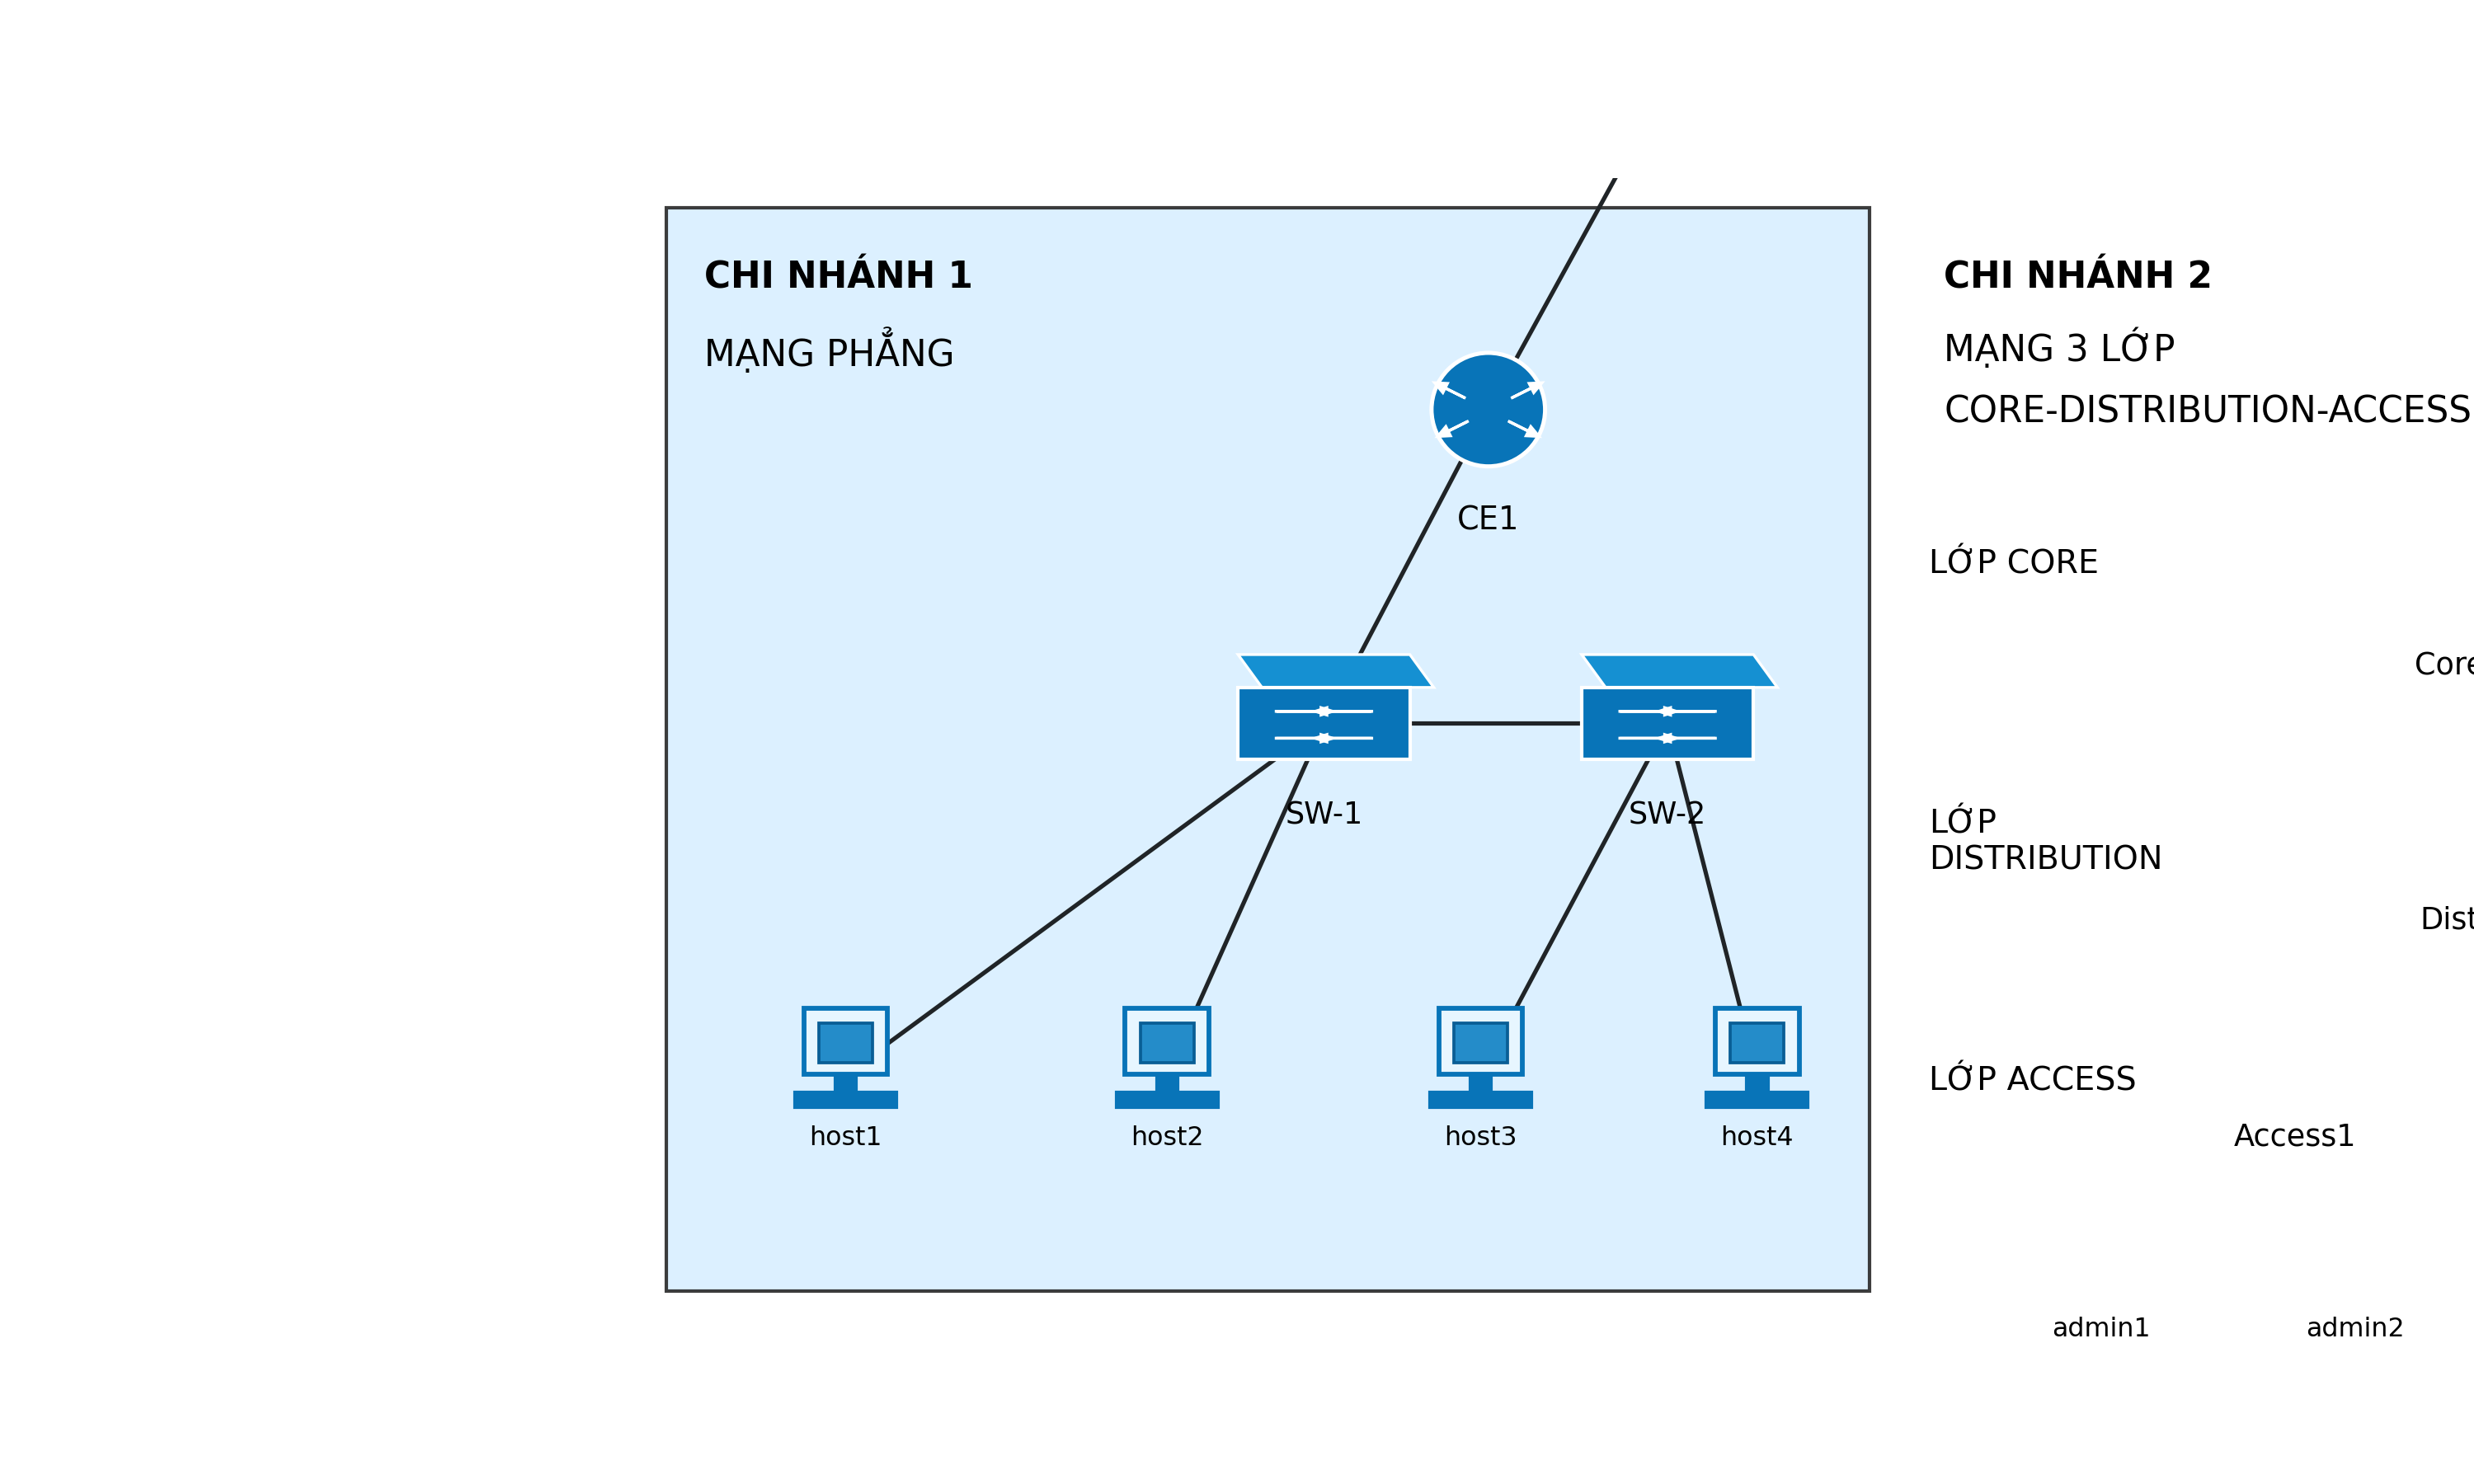
\includegraphics[width=0.88\linewidth]{image/branch1_flat.png}
    \caption{Branch 1 Flat Network}
\end{figure}

\subsection{Thiết kế Branch 2: Three-tier Network}

Branch 2 gồm các lớp access, distribution và core. Nhóm host gồm \texttt{admin1}, \texttt{admin2}, \texttt{user1}, \texttt{user2}, \texttt{guest1}, \texttt{guest2}, cùng subnet \texttt{10.2.0.0/24}. Gateway tại CE là \texttt{10.2.0.1}. Mục tiêu là mô phỏng mô hình LAN doanh nghiệp có phân tầng rõ ràng.

\begin{figure}[H]
    \centering
    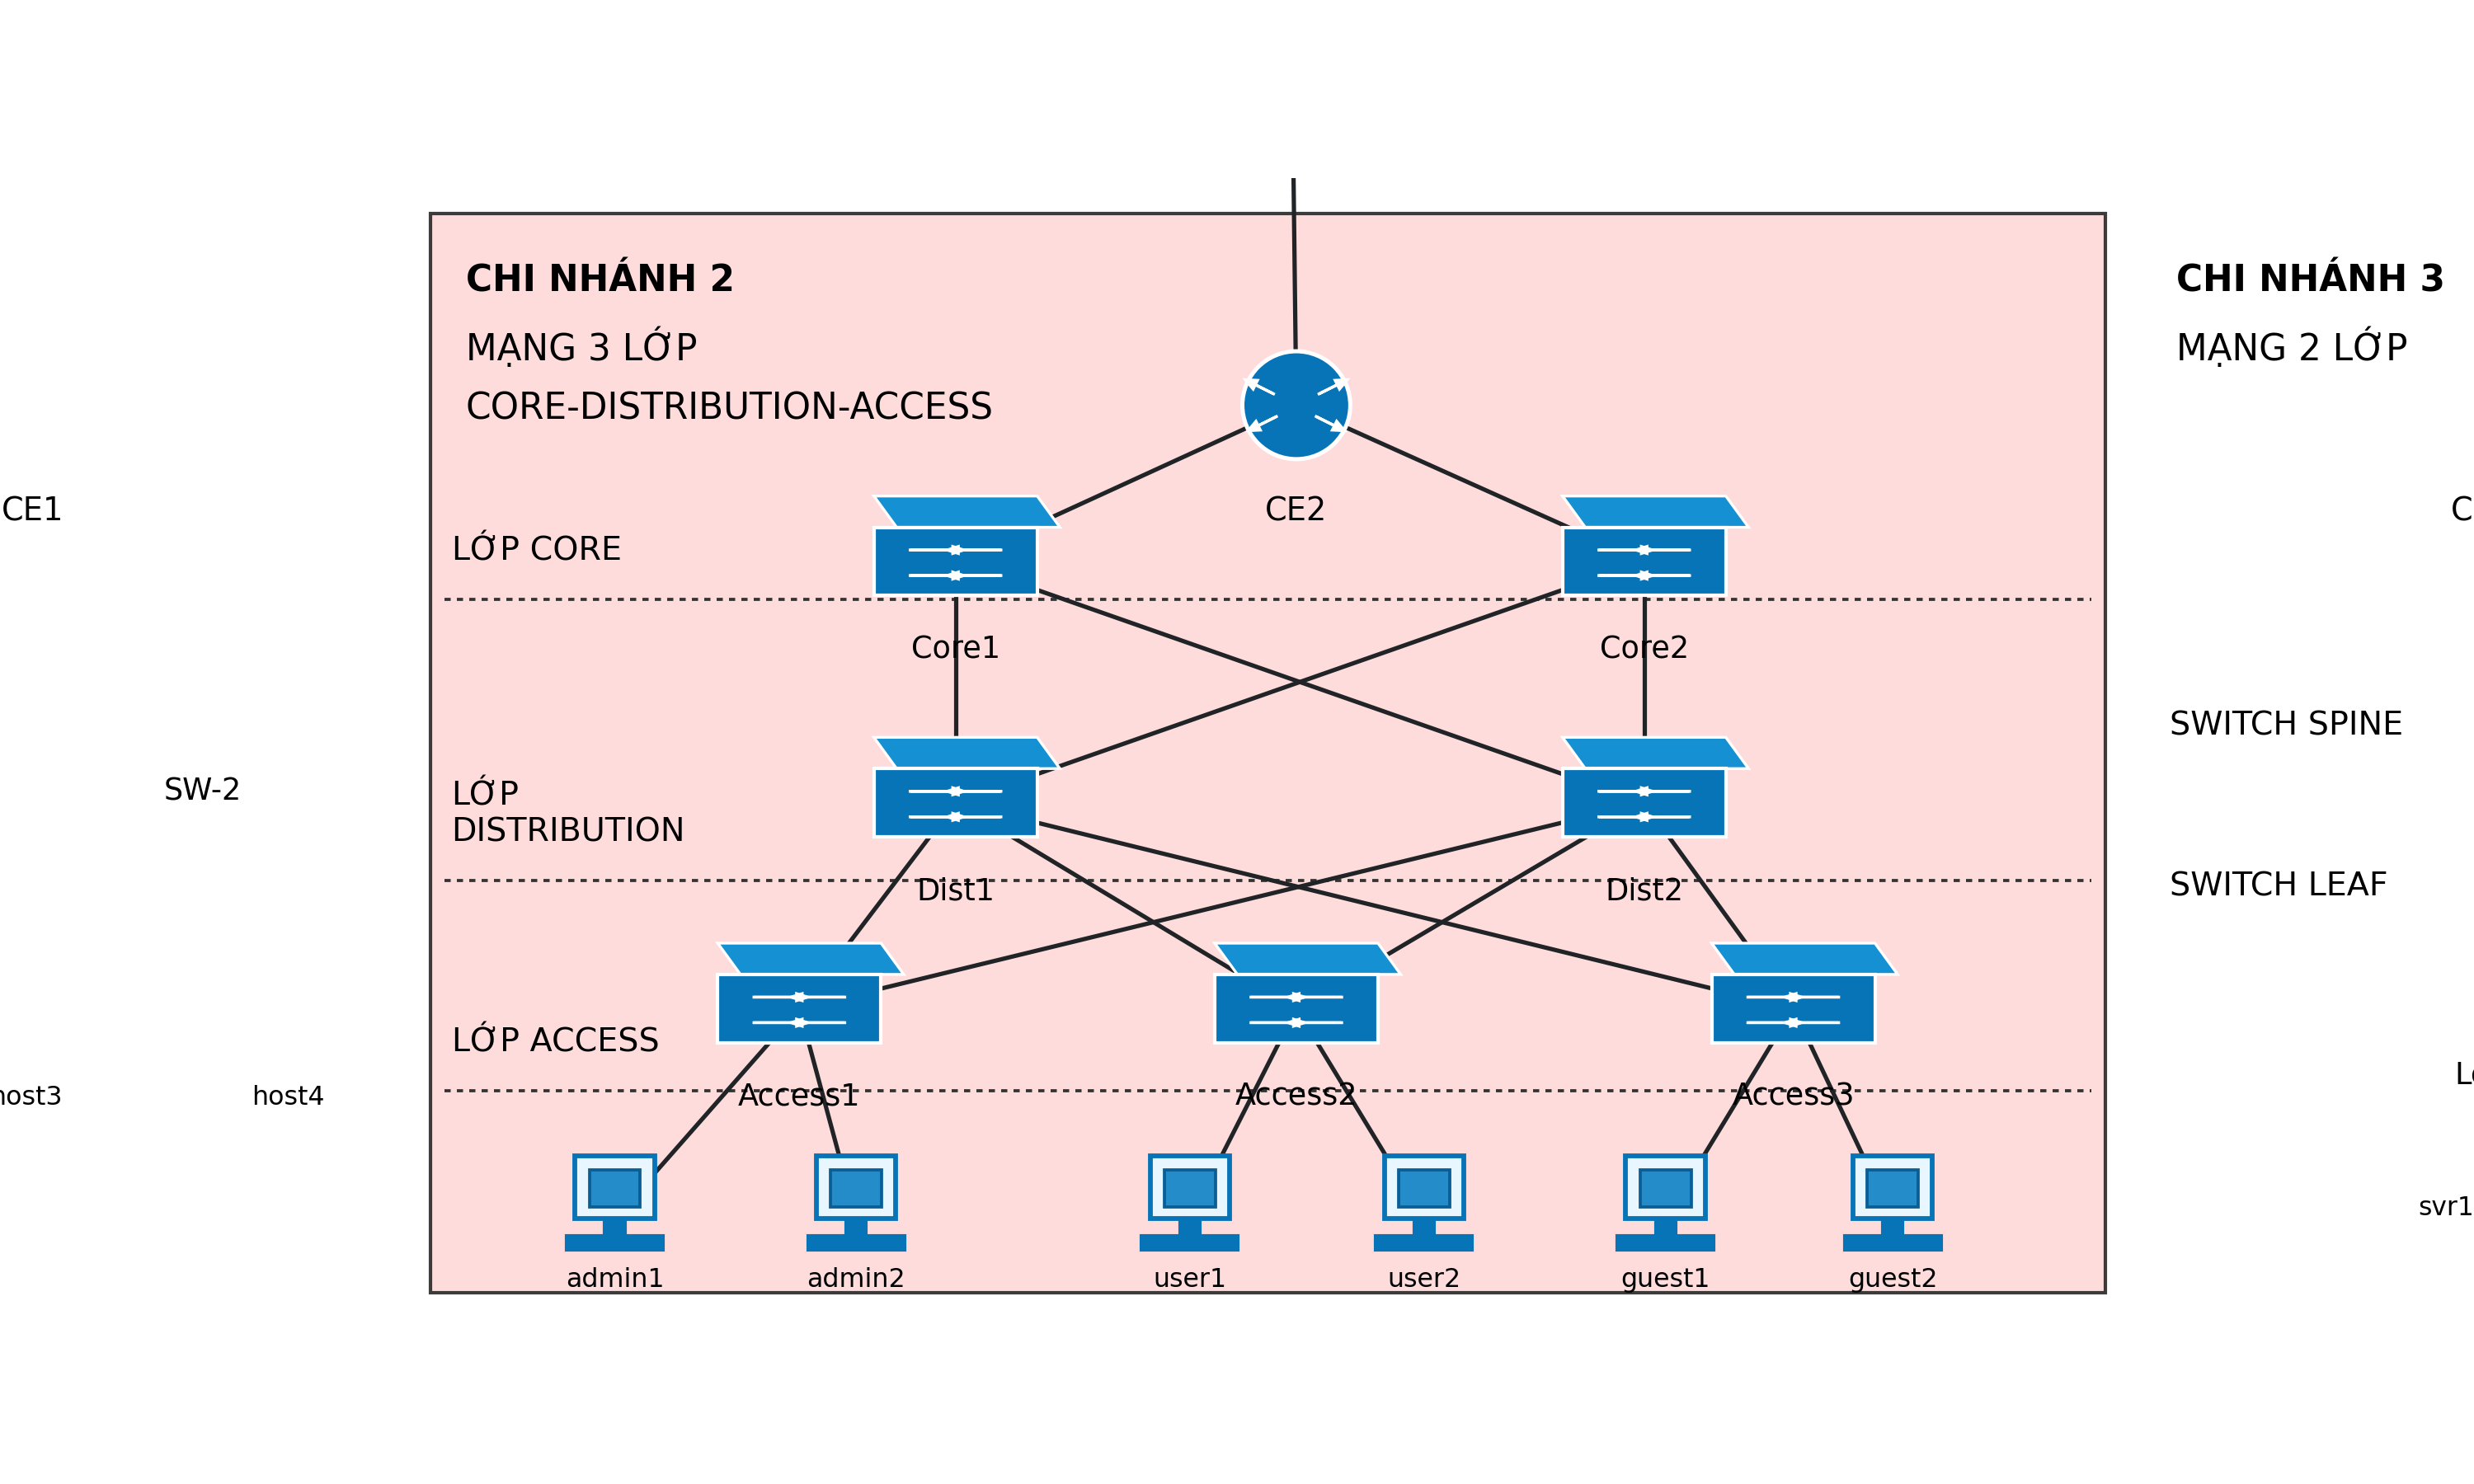
\includegraphics[width=0.9\linewidth]{image/branch2_three_tier.png}
    \caption{Branch 2 Three-tier Network}
\end{figure}

\subsection{Thiết kế Branch 3: Leaf-Spine Network}

Branch 3 gồm bốn leaf, hai spine, các server \texttt{svr1}, \texttt{svr2}, \texttt{svr3a}, \texttt{svr3b}, \texttt{svr4} và host \texttt{os1}, \texttt{os2}. Subnet chính là \texttt{10.3.0.0/24}, gateway là \texttt{10.3.0.1}. Topology được giữ loop-free ở Layer 2 để tránh phụ thuộc STP khi demo trên VM nhỏ.

\begin{figure}[H]
    \centering
    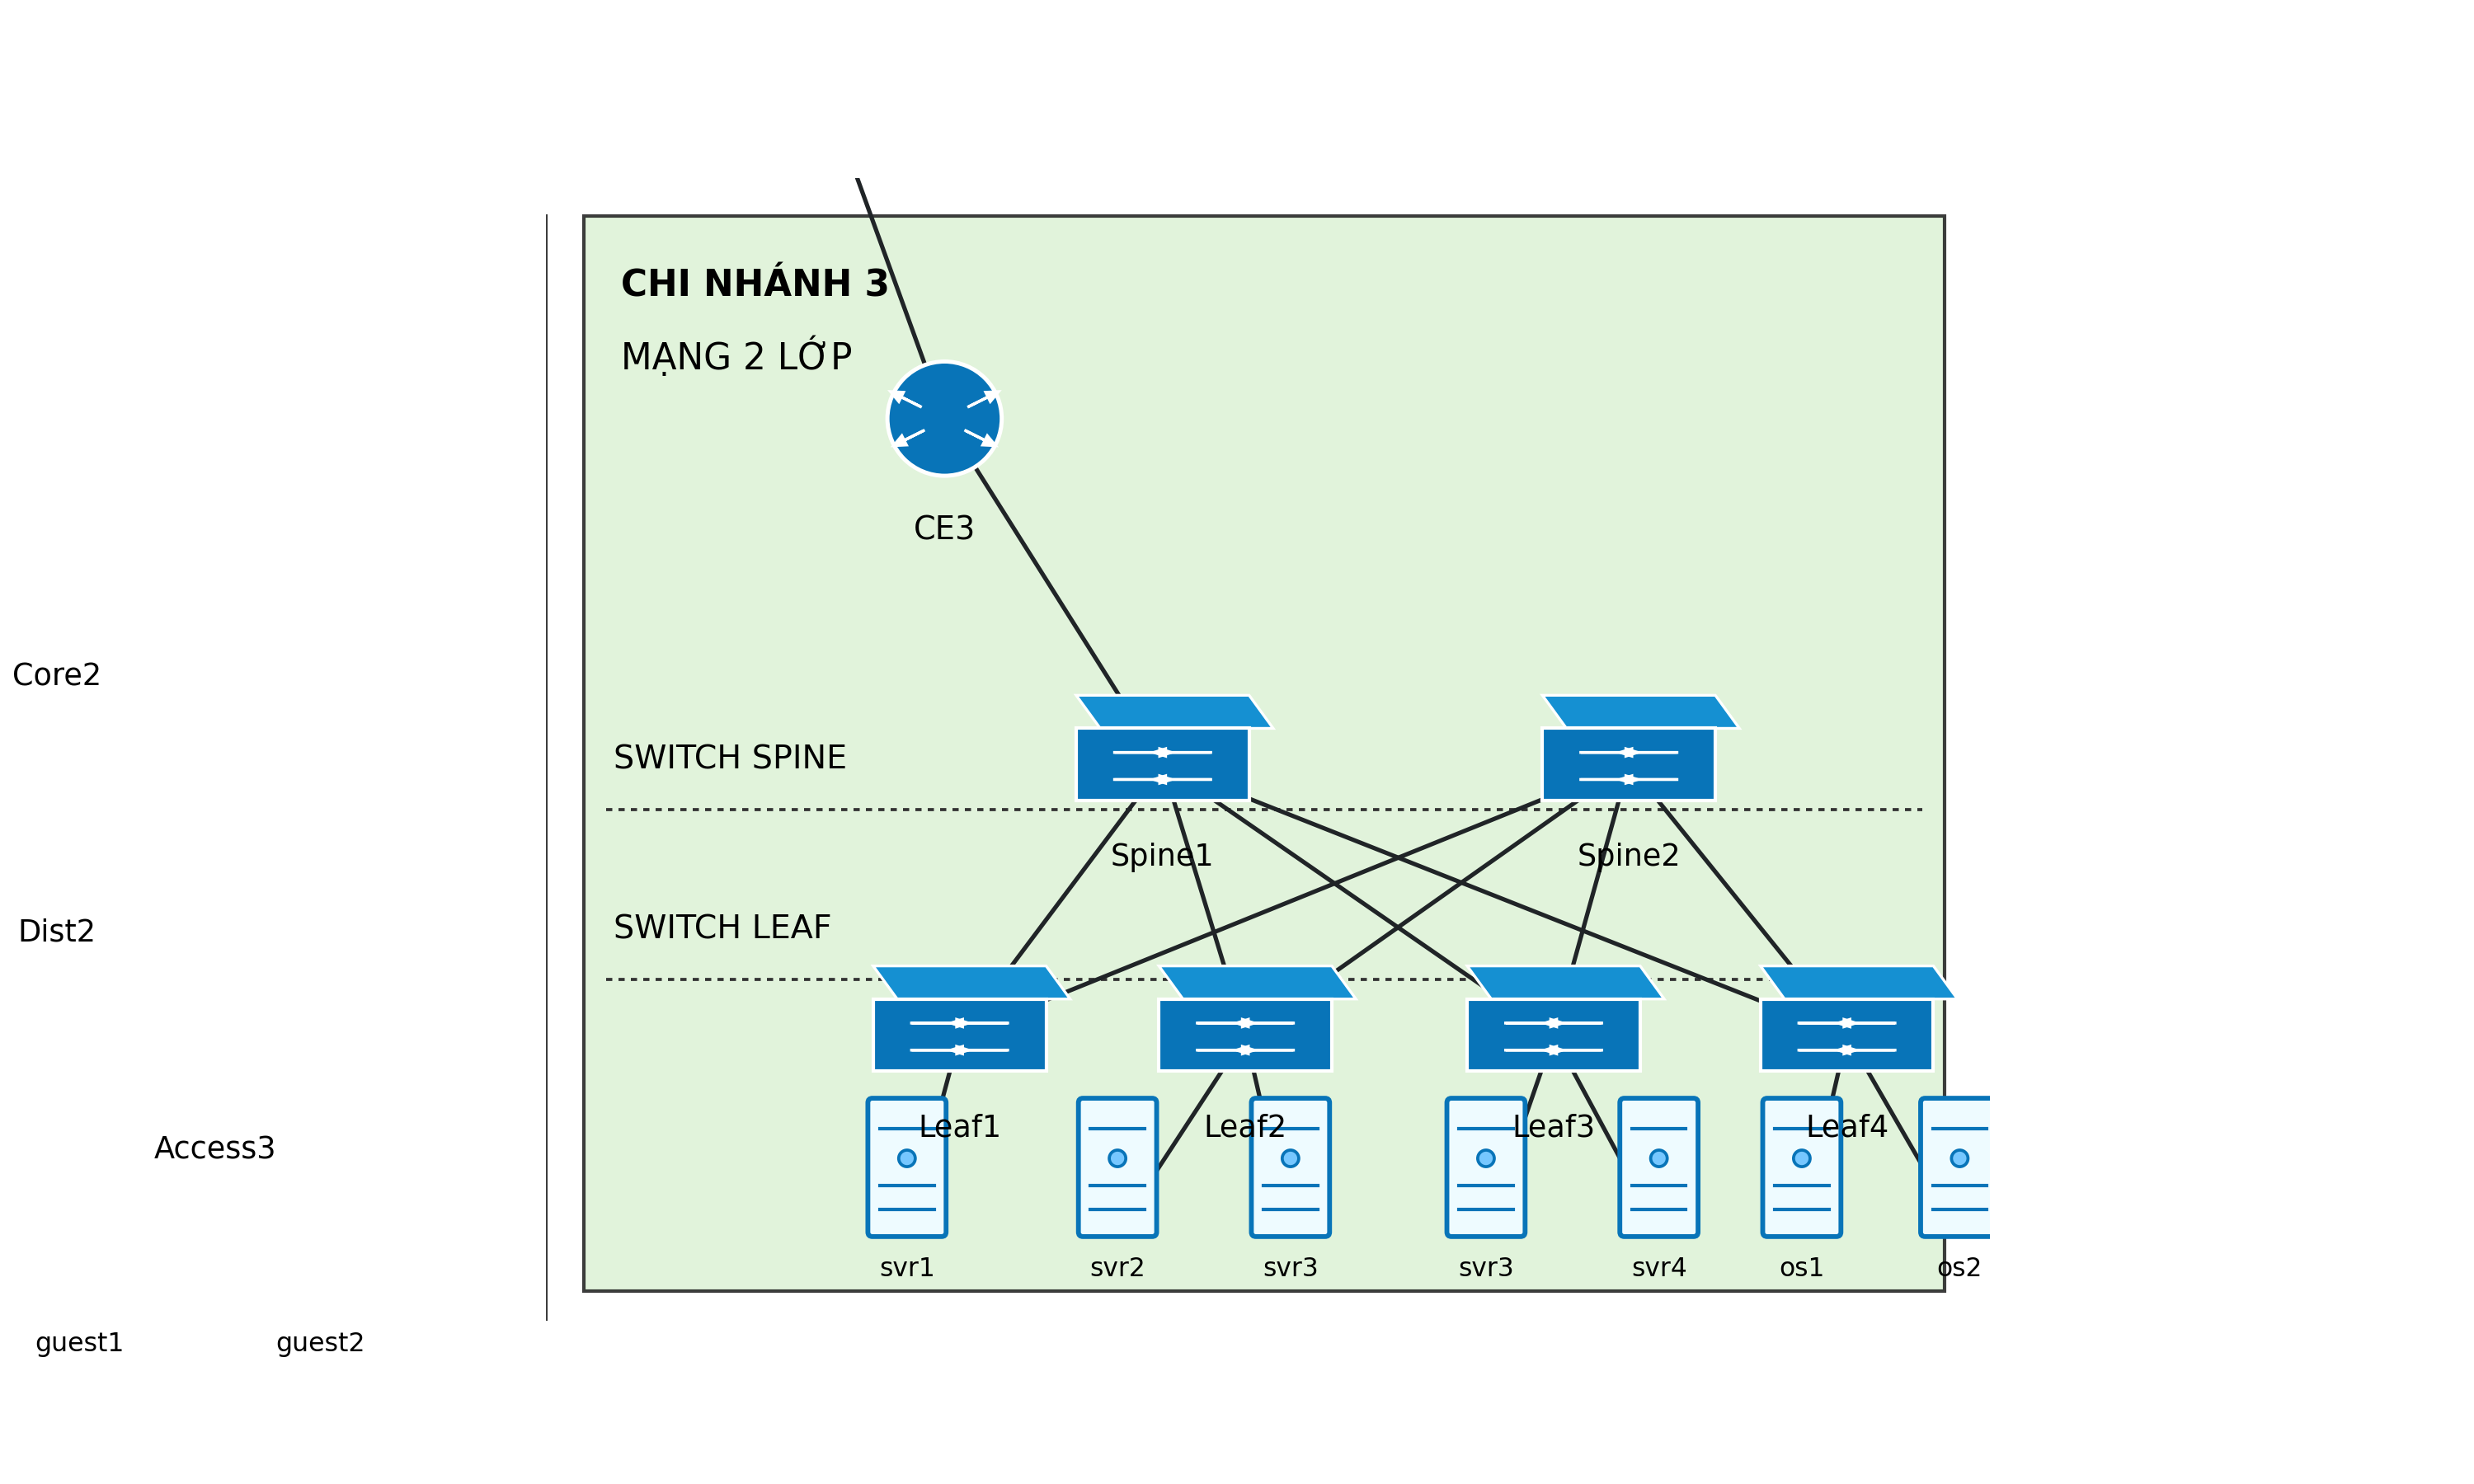
\includegraphics[width=0.9\linewidth]{image/branch3_leaf_spine.png}
    \caption{Branch 3 Leaf-Spine Network}
\end{figure}

\subsection{Thiết kế provider MPLS backbone}

Provider backbone gồm ba PE router: \texttt{pe1}, \texttt{pe2}, \texttt{pe3} và bốn P router: \texttt{p1}, \texttt{p2}, \texttt{p3}, \texttt{p4}. Các link CE-PE dùng băng thông 80 Mbps và delay 2 ms. Các link lõi PE-P và P-P dùng băng thông 50--60 Mbps, delay 3--4 ms để tạo khác biệt hiệu năng khi đo.

\begin{figure}[H]
    \centering
    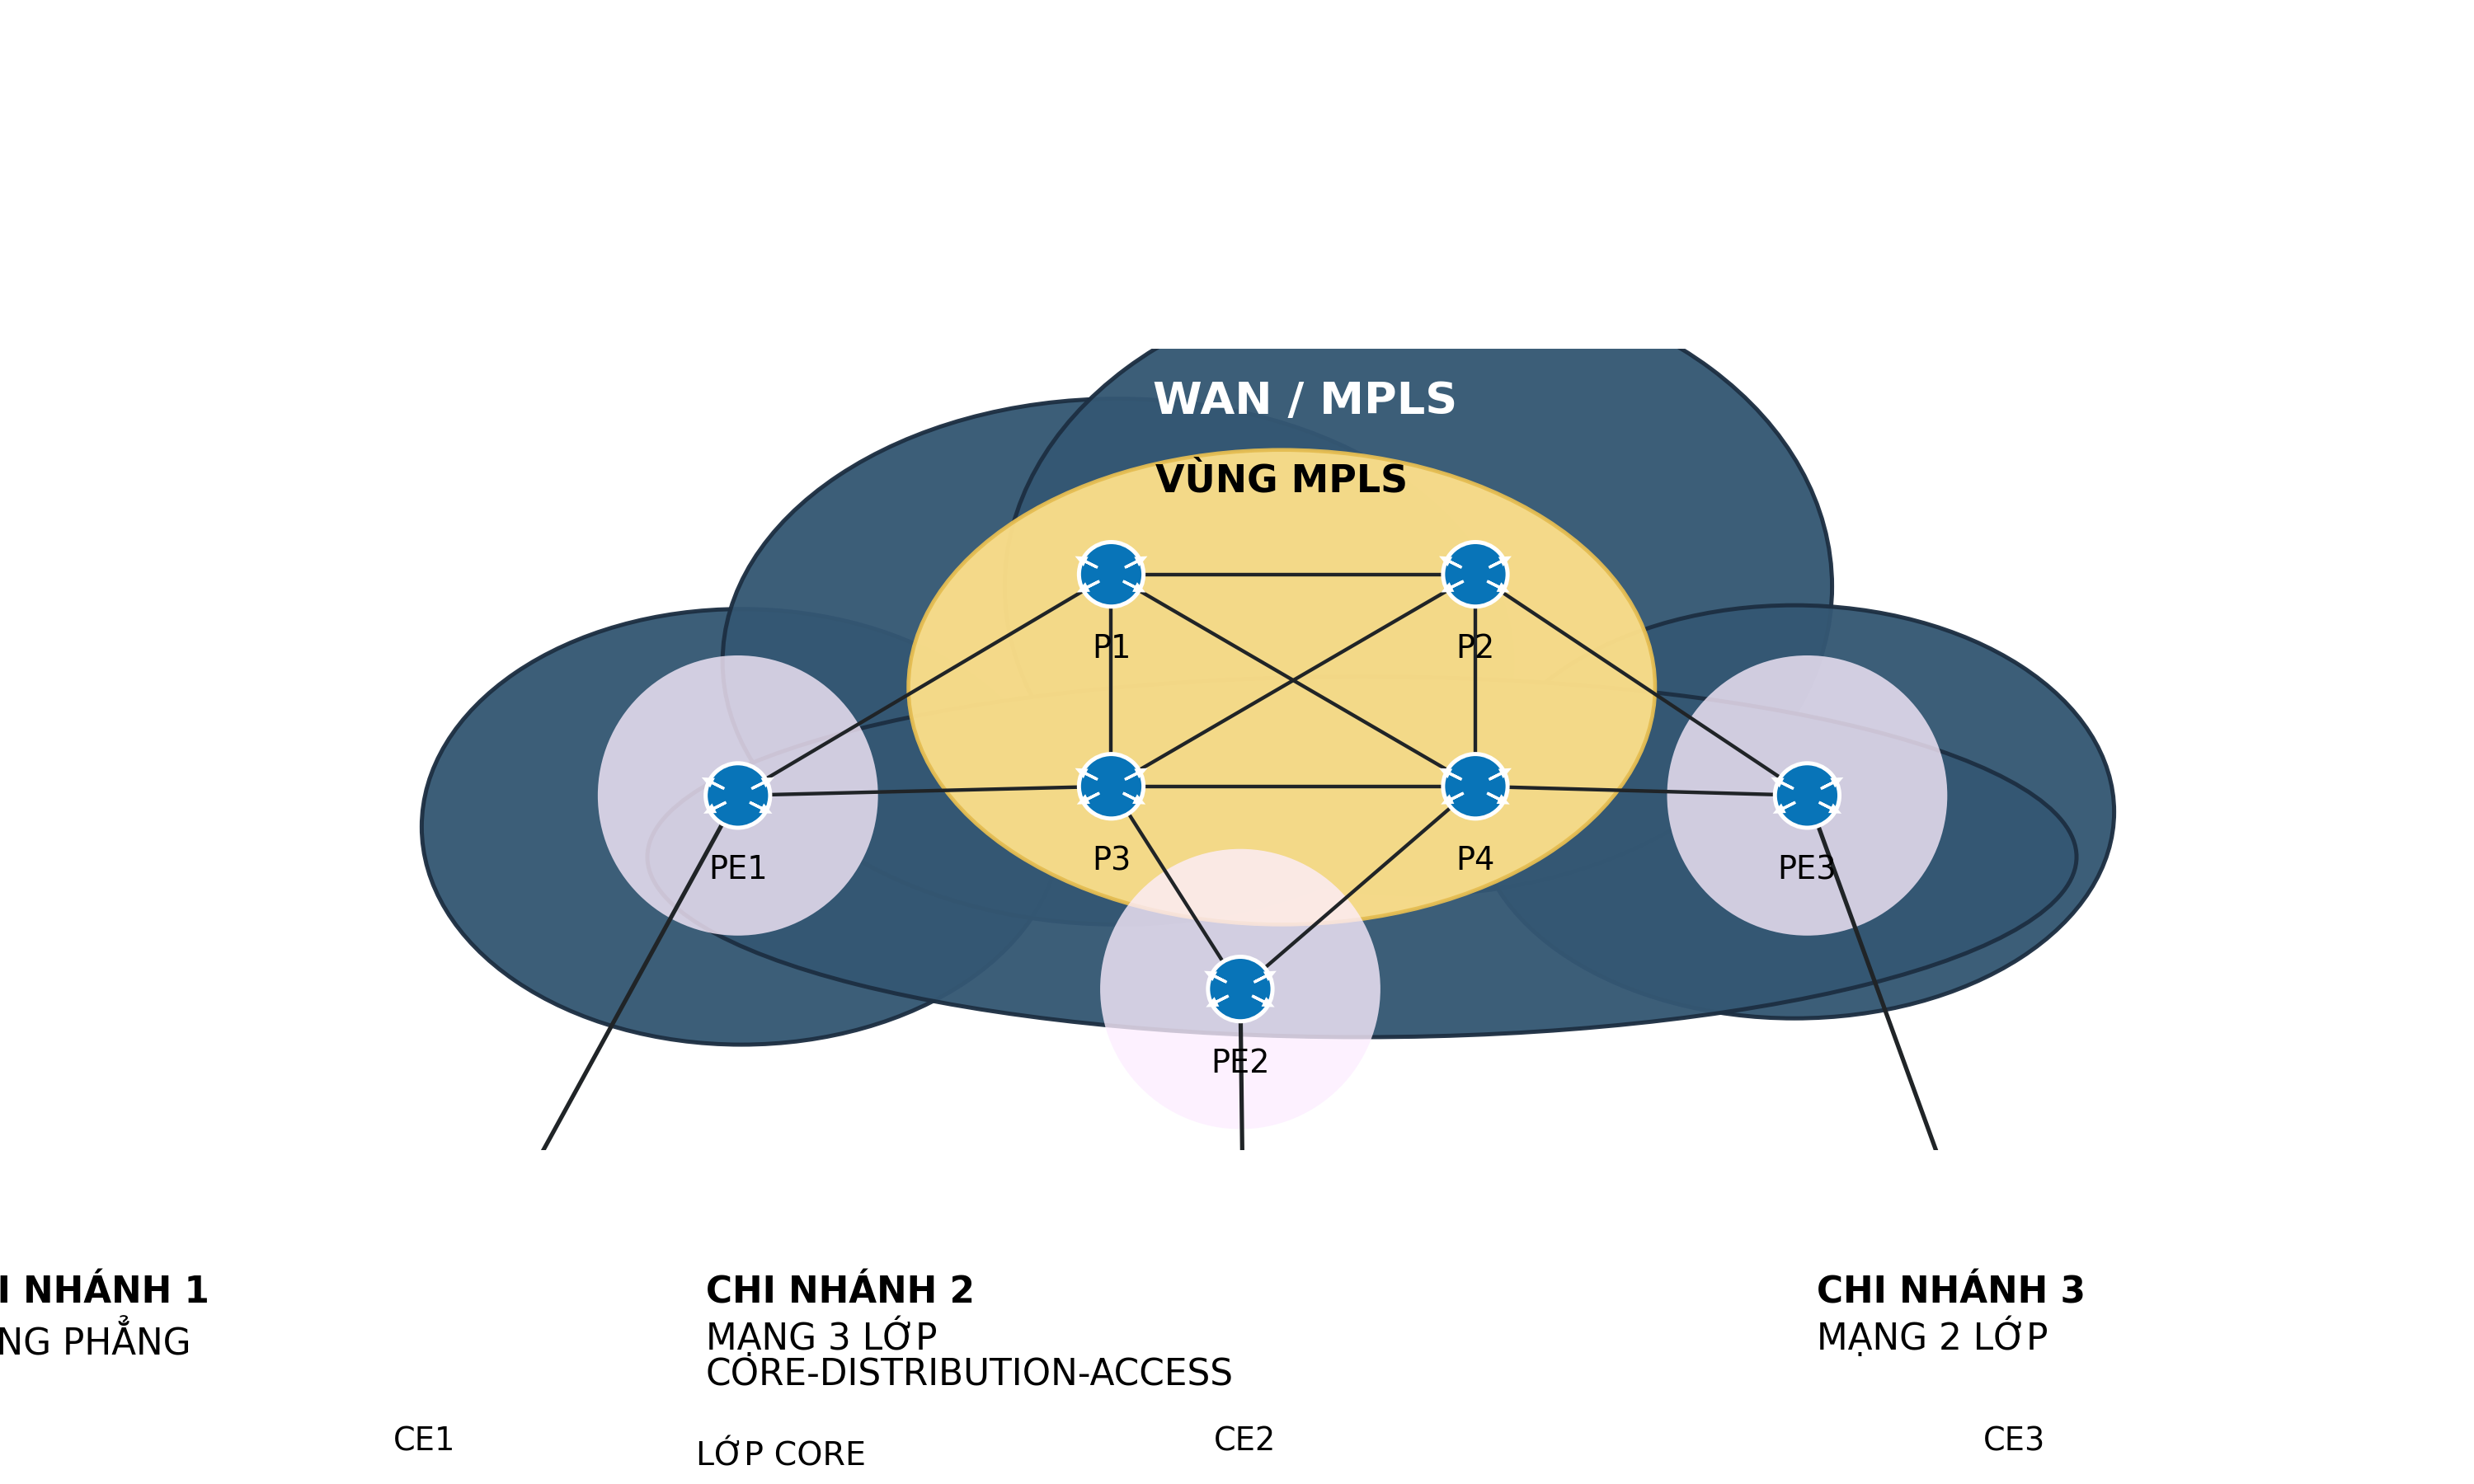
\includegraphics[width=0.9\linewidth]{image/mpls_backbone.png}
    \caption{Provider MPLS backbone}
\end{figure}

\subsection{Bảng địa chỉ chính}

\begin{table}[H]
\centering
\caption{Quy hoạch địa chỉ IP}
\begin{tabularx}{\linewidth}{|l|l|X|}
\hline
\textbf{Vùng mạng} & \textbf{Subnet} & \textbf{Ghi chú} \\
\hline
Branch 1 & 10.1.0.0/24 & Flat Network, gateway 10.1.0.1 \\
\hline
Branch 2 & 10.2.0.0/24 & Three-tier Network, gateway 10.2.0.1 \\
\hline
Branch 3 & 10.3.0.0/24 & Leaf-Spine Network, gateway 10.3.0.1 \\
\hline
CE-PE & 172.16.1.0/30, 172.16.2.0/30, 172.16.3.0/30 & Kết nối khách hàng với provider \\
\hline
Backbone & 172.20.0.0/30 & Các link PE-P và P-P \\
\hline
\end{tabularx}
\end{table}

\subsection{Logic đường đi gói tin}

Ví dụ luồng Branch 1 sang Branch 2:
\begin{enumerate}
    \item \texttt{host1} gửi gói đến gateway \texttt{b1\_ce}.
    \item \texttt{b1\_ce} route đến LAN Branch 2 qua CE remote \texttt{172.16.100.2}.
    \item Frame CE đi vào bridge VPLS/L2VPN trên \texttt{pe1}.
    \item Pseudowire GRETAP đưa frame sang PE remote; underlay đến loopback PE dùng route OSPF/LDP có nhãn MPLS.
    \item \texttt{pe2} giao frame ra \texttt{b2\_ce}, sau đó đến \texttt{user1}.
\end{enumerate}
